\chapter{Konzept (Anforderungen)}\label{konzept_2}
\section{Installation (UC-01)}\label{installation}
Zur Installation der Software benötigt man die Eclipse-Entwicklungsumgebung in der Version 3.7. Darin integriert befindet sich ein Update-Manager, der Software-Komponenten von Lokal oder dem Netzwerk installieren kann. Auch Updates werden über diesen Mechanismus installiert. Die Analyse-Software wird via eine Update-Seite bereitgestellt. Der Software-Build durch das Continuous Integration System publiziert die Artefakte (Features, Plugins) auf einen via Internet zugänglichen Server, von welchem der Update-Manager die Software herunterlädt um anschliessend zu importieren. Update-Seiten im Eclipse-Umfeld bestehen aus Features (Eclipse Feature-Projekt). Features bestehen aus unterschiedlichen Plugins (Eclipse Plugin-Projekt). Die Eclipse Runtime kann solche Softwarepakete zur Laufzeit installieren und updaten.

Die Update-Seite widerspiegelt die Struktur der Software:
\begin{itemize}
\item \textbf{Basissoftware:} Umfasst alle Plugins , die für die Basissoftware notwendig sind. Siehe Abschnitt \titleref{projektstruktur}.
\item \textbf{JRockit Erweiterung: }Umfasst alle Plugins zur JRockit Erweiterung und hat zugleich die Abhängigkeit auf das Basissoftware-Feature.
\end{itemize}

\section{Update (UC-02)}
Der Update eines Features auf der Update-Seite durch die Erstellung eines neuen Releases ist erkennbar durch eine Änderung der Versionsnummer. Beim Starten der Software wird überprüft, ob ein sich auf dem Server befindendes Feature aktualisiert wurde. Der Benutzer kann diese im laufenden Betrieb der Applikation installieren, ein Neustart ist allerdings danach Pflicht.

\section{Datei importieren (UC-03)}
Der Import\footnote{Der Begriff Import ist irreführend, da diese Aktion einzig dazu dient, die Datei in die Ansicht Logdateien zu kriegen. Erst mit dem Öffnen der Datei werden die Daten wirklich gelesen.} einer Logdatei findet über einen Import-Wizard statt. Der Ablauf ist folgendermassen:
\begin{enumerate}
	\item Import-Wizard öffnen
	\item Auswahl des Ordners
	\item Selektion einer oder mehrerer Logdateien
	\item Bestätigung der Eingaben
	\item Anschliessend wird die Logdatei als Instanz von \textit{IFileDescriptor} in der Ansicht \textit{Logdateien} angezeigt, der Inhalt wurde allerdings noch nicht analysiert.
\end{enumerate}

\subsection{Importierte Dateien speichern (UC-03.1)}
Der im Abschnitt \ref{memento} beschriebene Mechanismus wird verwendet, damit nach einem Neustart der Entwicklungsumgebung die importierten Logdateien nicht verloren gehen. 

\section{Datei einlesen (UC-04)}
Durch den Import einer Garbage Collection Logdatei erscheinen diese im Fenster \textit{Logdateien}. Das öffnen einer dieser Dateien lädt den Inhalt in den Arbeitsspeicher. Die Daten sind noch unstrukturiert und werden innerhalb des im nächsten Abschnitt definierten Domänenmodells gespeichert.

\subsection{Domänenmodell}
\textit{IFileDescriptor} wird für die Abstraktion der Garbage Collection Logdatei verwendet. Darin enthalten sind Metadaten wie Dateiname und Pfad sowie - wenn bereits geladen - der Inhalt der Datei. Die Abstraktion einer Garbage Collection Logdatei heisst \textit{AbstractJvmRun} und wird erst von der jeweiligen Erweiterung realisiert.
 \begin{figure}[H]
  	\centering
    	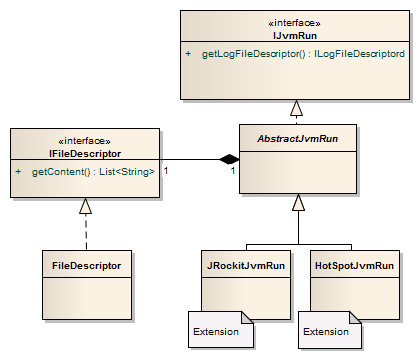
\includegraphics[width=16cm]{images/core_domain}
        	\caption{Domänenmodell: Eingelesene Datei}
\end{figure}

\section{Logdatei parsen (FRQ-05)}
Die Garbage Collection Logs der JRockit Virtual Machine bestehen aus Einträgen unterschiedlicher Log Module. Diese Ausgaben können selektiv per Kommandozeile aktiviert werden (siehe Abschnit \ref{logmodule}). Für die Garbage Collection Analyse sind nicht alle Einträge relevant, es werden nur die wichtigsten verwendet. Die einzelnen Parser für die Garbage Collection Logdatei werden auf der Basis von Regular Expressions selber implementiert. Auf die Verwendung eines Parser-Generators wird aus folgenden Gründen verzichtet:
\begin{itemize}
	\item Lightweight: Um Parser-Generatoren zu verwenden, wird in der Regel auch zur Laufzeit eine Bibliothek benötigt. Diese muss mit der Software ausgeliefert werden. Die Implementation eines Parser auf der Basis von Regulären Ausdrücken kann mit Java Standardmitteln gemacht werden.
	\item Proprietär: Parser-Generatoren sind proprietär und die Verwendung dessen bedingt gute Kenntnisse. In der Regel beschreibt man das Format in einer Grammatik.
\end{itemize}

\subsection{Parser}
Der Parser für die Logdateien der JRockit Virtual Machine ist nach dem Chain-of-Responsibility Pattern\cite{wiki:chainOfResponsibilityPattern} aufgebaut. Pro Log-Eintrag (respektive pro Typ eines Log-Eintrags) kann ein Parser in die Parser-Kette geschaltet werde. Jeder Parser extrahiert die für ihn wichtigen Informationen und aktualisiert damit das Domänenmodell. Die wichtigsten Einträge der Garbage Collection Logdatei sind die des Memory Modules und werden vom \textit{MemoryModuleParser} verarbeitet. In zukünftigen Versionen ist die Verarbeitung von Log-Einträgen von anderen Log-Modulen denkbar - Einträge des Nursery- oder Allocation-Modules, etc. Ablauf und Aufbau des Parsers sind in den folgenden beiden Grafiken ersichtlich:

 \begin{figure}[H]
  	\centering
    	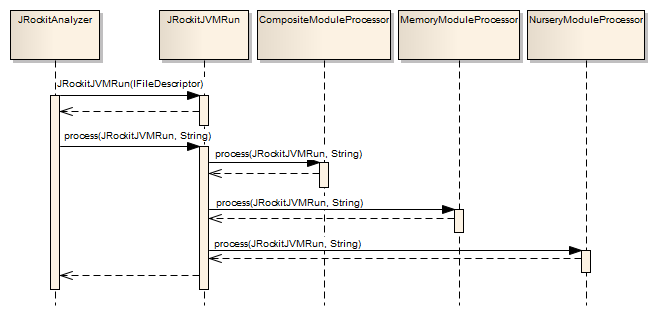
\includegraphics[width=16cm]{images/acitivity_parse_prozess}
        	\caption{Sequenzdiagramm Parser}
\end{figure}
 \begin{figure}[H]
  	\centering
    	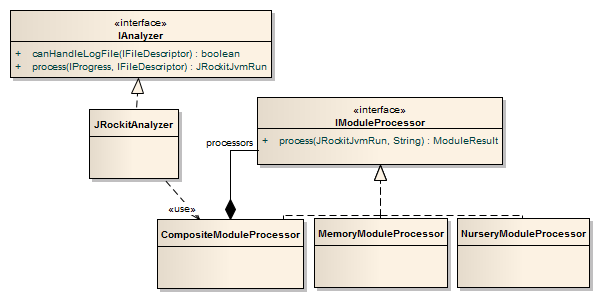
\includegraphics[width=16cm]{images/jrockit_log_processing}
        	\caption{Klassendiagramm Parser}
\end{figure}

\subsection{MemoryModuleParser}
Das Parsen innerhalb des \textit{MemoryModuleParser} wird in zwei Schritte aufgeteilt:
\begin{itemize}
\item \textbf{Lexer: }Der einzelne Logeintrag wird durch den Lexer (Tokenizer) in eine Map aus Tokens umgewandelt. Schlüssel für die einzelnen Tokens ist der \textit{TokenType}. Der Lexer wird mittels Regular Expressions implementiert. Die Werte werden mittels Gruppierungs-Funktion\footnote{Mittels Gruppen innerhalb von Regulären Ausdrücken lassen sich einzelne Werte aus einem String extrahieren.} extrahiert. 
\item \textbf{Syntactic Analyzer: }Der syntaktische Analyser verarbeitet die vom Lexer extrahierten Tokens. Er führt zum einen eine semantische Validierung durch und speichert die Werte in strukturierter Form (Domänenmodell).
\end{itemize}

\subsection{Auswertung Logdatei}
Bereits in Abschnitt \ref{logexample} ist ein Teil einer Garbage Collection Logdatei aufgelistet. Dieser Abschnitt zeigt die für die Garbage Collection Analyse wichtigsten Informationen und Auswertungen die mit der Analysesoftware dafür gemacht werden können, ohne dabei aber auf die Ausgaben des Debug-Log-Levels\footnote{Der Log-Level kann für jeden einzelnen Logger eingstellt werden.} einzugehen.

\subsubsection{Garbage Collection Algorithmus}
\begin{lstlisting}[numbers=none,  framexleftmargin=0mm, caption=Logdatei: Ausgabe initialer Garbage Collection Algorithmus]
[INFO ][memory ] GC mode: Garbage collection optimized for throughput, strategy: Generational Parallel Mark & Sweep.
\end{lstlisting}
Die eigentlich wichtigste Information respektive Entscheidung zum Garbage Collection Tuning ist die Wahl der Strategie. Sie wird im Header der Logdatei angezeigt und entspricht entweder der Standardeinstellung oder wird konfiguriert. Ausgewertet aus dem Eintrag werden zwei Dinge: für was die Garbage Collection optimiert ist (Durchsatz oder Pausenzeiten) und die Strategie (Generational Parallel Mark \& Sweep, Parallel Mark \& Sweep, Genertional Concurrent Mark \& Sweep, Concurrent Mark \& Sweep).
	
\subsubsection{Initiale und maximale Heap-Kapazität, Grösse Old- und Young-Space}
\begin{lstlisting}[numbers=none,  framexleftmargin=0mm, caption=Logdatei: Initiale und maximale Heap-Kapazität und Grösse des Old- und Young-Spaces]
[INFO ][memory ] Heap size: 65536KB, maximal heap size: 1048576KB, nursery size: 32768KB.
\end{lstlisting}
Ebenfalls im Header der Logdatei befindet sich die Angabe über die initiale und maximale Heap-Kapazität und die grösser des Young-Spaces (Nursery). Die grösse des Old-Spaces (Tenured Space) errechnet sich aus der Differenz zwischen Young-Space und maximaler Kapazität.

\subsubsection{Young-Collection Information}
\begin{lstlisting}[numbers=none,  framexleftmargin=0mm, caption=Logdatei: Information Young-Collection]
[INFO ][memory ] [YC#660] 2.172-2.172: YC 200108KB->200147KB (233624KB), 0.001 s, sum of pauses 0.536 ms, longest pause 0.536 ms.
\end{lstlisting}
Der Abschluss einer Young-Collection wird mit dem oben aufgelisteten Log-Eintrag dokumentiert. Er beschreibt Start- und Endzeitpunkt sowie die Grösse des Heaps vor und nach der Garbage Collection. Des weiteren ist die Dauer, die Summe aller einzelnen Pausen und die längste Pause aufgelistet. 

\subsubsection{Old-Collection Information}
\begin{lstlisting}[numbers=none,  framexleftmargin=0mm, caption=Logdatei: Information Old-Collection]
[INFO ][memory ] [OC#3] 2.544-2.733: OC 233624KB->187955KB (280628KB), 0.189 s, sum of pauses 187.019 ms, longest pause 187.019 ms.
\end{lstlisting}
Die Ausgabe einer Old-Collection unterscheidet sich, ausgenommen vom Typ (OC),  nicht von der einer Young-Collection.

\subsubsection{Wechsel der Garbage Collection Strategie}
\begin{lstlisting}[numbers=none,  framexleftmargin=0mm, caption=Logdatei: Wechsel Garbage Collection Strategie]
[INFO ][memory ] [OC#6] Changing GC strategy from: singleconpar to: singleconcon, reason: Return to basic strategy.
\end{lstlisting}
Aus unterschiedlichen Gründen kann es zu einem Wechsel der Garbage Collection Strategie kommen. Dieser wird, zusammen mit dem Grund für den Wechsel, in der Logdatei dokumentiert und kann ausgewertet werden.


\subsection{Domänenmodell JRockit Garbage Collection}\label{jrockit_domain_model}
Der Parseprozess wandelt die unstrukturierten Daten in ein strukturiertes Domänenmodell um. Dieses wurde wie folgt erarbeitet:
\begin{landscape}
 \begin{figure}[H]
  	\centering
        	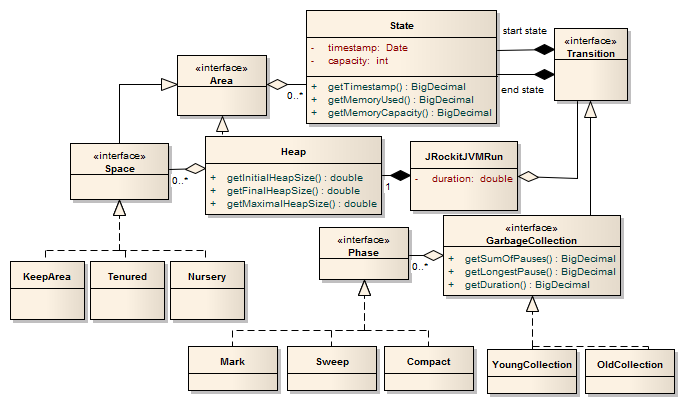
\includegraphics[width=16.6cm]{images/jrockit_extension_domain}
	\caption{Domänenmodell: Garbage Collection (JRockit Implementation)}
\end{figure}
\end{landscape}
Die Daten der Logdatei repräsentieren einen Lauf einer JVM (\textit{JRockitJVMRun}) bestehend aus einem Heap und den darin enthaltenen Bereichen Keep-Area, Nursery und Tenured Space. Jeder dieser Bereiche hat unterschiedliche Zustände welche durch die Logdatei repräsentiert werden. Die Daten sind also nicht zu jedem Zeitpunkt, sondern nur für diese Zustände bekannt. Übergänge finden durch Transitionen respektive durch eine Garbage Collection statt, es kann sich dabei um Young oder Old Collections handeln. Das starten einer Transition wird durch einen Event ausgelöst (hier im Diagramm nicht ersichtlich), Events werden aufgrund von heuristischen Daten der Lauzeitumgebung ausgelöst - zum Beispiel wenn die Nursery oder die Old Collection an ihre Speichergrenze gelangen. Der Vollständigkeit halber sind im Diagramm zusätzlich noch die einzelnen Phasen der Garbage Collection definiert, die bei einer Garbage Collection durchlaufen werden.

\section{Standardauswertung anzeigen (FRQ-06)}
\subsection{Anzeige Übersicht Garbage Collection (FRQ-06.1)}\label{standardreport}
Der initiale Tab der Analyseseite zeigt eine Zusammenfassung der geöffneten Garbage Collection Logdatei. Die Daten werden in den Tabellen Heap Kapazität, Garbage Collection Aktivität und Gesamtstatistik angezeigt:

\subsubsection{Heap Kapazität}
\begin{itemize}
	\item Initiale und maximale Heap Kapazität
	\item Grösse Young- und Old-Space
	\item Speicherbedarf Peak, Durchschnitt: Aus den Informationen des Speicherverbrauchs vor und nach jeder Garbage Collection wird der durchschnittliche und der maximale Bedarf berechnet.
	\item Kapazität Peak, Durchschnitt: Aus den Informationen der Kapazität vor und nach jeder Garbage Collection wird die durchschnittliche und maximale Kapazität des Heaps berechnet.

\end{itemize}
\subsubsection{Garbage Collection Aktivität (Young und Old Collection)}
\begin{itemize}
	\item Letzte Garbage Collection: Zu welchem Zeitpunkt hat die letzte Garbage Collection statt gefunden.
	\item Anzahl Garbage Collections: Wieviele Garbage Collections hat es insgesamt gegeben.
	\item  Anzahl Old Collections: Wieviele Old Collections hat es gegeben.
	\item Anzahl Young Collections: Wieviele Young Collections hat es gegeben.
	\item Total Zeit der Garbage Collection: Totale Zeit, in welcher sich die Virtual Machine in der Garbage Collection befunden hat.
	\item Durchsatz der Applikation (siehe Abschnitt \ref{gc_tuning_durchsatz})

	\item Durchschnittlicher Interval in Sekunden: Durchschnittliche Pausenzeit zwischen den einzelnen Garbage Collections
	\item Durchschnittliche Dauer in Sekunden
	\item Totale Zeit der Old Garbage Collection Zyklen
	\item Totale Zeit der Young Garbage Collection Zyklen
	\item Prozentuale Zeit der Old Garbage Collection Zyklen
	\item Prozentuale Zeit der Young Garbage Collection Zyklen
\end{itemize}	

\subsubsection{Gesamtstatistik}
\begin{itemize}
	\item Dauer der Messung in Sekunden
\end{itemize}

\subsection{Chart Anzeige Heap Benutzung (FRQ-06.2)}
Die Heap-Analyse zeigt den Verlauf des benutzten \textbf{Speichers} im Heap über die Zeit auf. Die einzelnen Garbage Collection Zyklen (Young, Old) werden verschiedenfarbig dargestellt.

\subsection{Chart Anzeige Dauer Garbage Collection (FRQ-06.3)}
Die \textbf{Dauer} der einzelnen Garbage Collection Zyklen wird über die Zeit aufgezeigt. Die einzelnen Garbage Collection Zyklen (Young, Old) werden verschiedenfarbig dargestellt.

\section{Profil erstellen (UC-07)}
Die Ansicht Profile zeigt die vom Benutzer erstellten Profile\footnote{Initial befindet sich darin allerdings nur das Standard-Profil.}. Die Beschreibung eines Analysefensters (Name, Beschreibung, Charts mit Serien, etc.) wird anhand von Profilen definiert. Es gibt folgende zwei Arten:
\begin{itemize}
	\item \textbf{Unveränderliches Profil:} Das Standard-Profil ist aktuell das einzige unveränderliche Profil. Es wird durch die \textit{JRockit Extension} definiert und kann nicht konfiguriert, verändert werden.
	\item \textbf{Veränderliches Profil:} Ein veränderliches Profil wird zur Speicherung des vom Benutzer definierten Analysefensters verwendet. Alle Änderungen die der Benutzer am Analysefenster macht (Chart hinzufügen, Chart konfigurieren), werden via ein Data-Binding an das Profil propagiert. Durch das Speichern des Profils hat der Benutzer die Möglichkeit, die selbe Analyse auch zu einem späteren Zeitpunkt an der gleichen oder einer anderen Logdatei durchzuführen.
\end{itemize}

\subsection{Domänenmodell zur Persistierung der Profile}
\textit{IConfiguration} dient zur Gruppierung von Profilen. Pro Extension wird eine Konfiguration mit verschiedenen Profilen abgelegt. Innerhalb eines Profils können unterschiedliche Diagramme (\textit{IChart}) angelegt werden, welche wiederum durch Achsen (\textit{IAxis}) und deren Datenquellen \textit{IValueProvider} definiert sind. \textit{IValueProvider} definieren den Weg, wie die Daten aus dem Domänenmodell ins Chart gelesen werden.
 \begin{figure}[H]
  	\centering
    	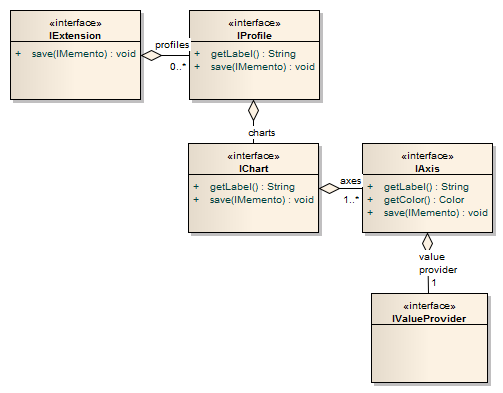
\includegraphics[width=11cm]{images/core_domain_profiles}
        	\caption{Domänenmodell: Profile}
\end{figure}

\subsection{Charts definieren (UC-07.1)}
Bei der Benutzung eines veränderlichen Profils hat der Benutzer die Möglichkeit, dem Analysefenster weitere Charts respektive Diagramme hinzuzufügen oder aber bereits existierende Diagramme zu manipulieren (weitere Serien hinzufügen, Serien entfernen, etc.). Die Manipulationen des Benutzers finden auf den Chart-Objekten statt und werden durch das Data-Binding propagiert. Die Administrationsoberfläche für einen Chart umfasst initial zwei Abschnitte:
\begin{itemize}
	\item Serie erstellen, definieren und hinzufügen
	 \item Serie löschen
\end{itemize}

\subsection{Profil speichern (UC-07.2)}
Mittels des Memento-(siehe Anhang \ref{memento}) und Visitor-Patterns\cite[S. 331]{gamma1995design} werden die Profile gespeichert.

\subsection{Profil exportieren, importieren (UC-07.3/ UC-07.4)}
Die Analysesoftware stellt zum Sichern und Verteilen von Profilen einen Import-Export-Mechanismus bereit. Beide sind in den Eclipse Standard-Wizards ersichtlich oder können via rechtem Mouseklick (Ansicht Profile) gestartet werden. Der Profile-Export und -Import basiert wie das Speichern auf dem im Abschnitt \ref{memento} beschriebenen Memento-Mechanismus. Zur Serialisierung in eine Datei wird das XMLMemento verwendet. 

\subsection{Hilfesystem (UC-08)}
Das Hilfesystem der Eclipse Entwicklungsumgebung ist als Client-Server-Lösung implementiert. Beim Start der Entwicklungsumgebung wird zusätzlich ein Jetty-Server gestartet, der die Hilfedienste wie Suche und Indexierung bereitstellt. Hilfeseiten sind auf unterschiedliche Weise verfügbar:
\begin{itemize}
\item \textbf{Indexbasierte Hilfen:} Für die generellen Informationen und Hilfen werden verschiedene Hilfeseiten basierend auf einem Index bereitgestellt. Die Inhalte sind nicht an ein Fenster oder eine Aktion des Benutzers gebunden. 
\item \textbf{Kontextsensitive Hilfen:} Tipps die im Zusammenhang mit einer Aktion oder eines Fensters stehen werden mit den kontextsensitiven Hilfen implementiert.
\end{itemize}

%--------------------------------------------
\section{Testabdeckung (QRQ-S-02)}\label{testing}
Bei Plugin-Projekten wird der Test-Code normalerweise in eigenen Fragment-Projekten abgelegt. Diese Test-Projekte werden allerdings nicht mit dem Feature ausgeliefert, sondern nur während dem Testen verwendet. Der Zugriff auf den Code der Implementation wird gewährleistet, indem aus dem Test-Projekt ein Fragment\footnote{Fragmente haben vollen Zugriff auf ihre Host-Bundles.} gemacht wird. Als Testing-Framework wird der defakto Standard JUnit verwendet. JUnit ist sowohl von allen Entwicklungsumgebungen als auch von Maven und Tycho unterstützt.

\section{Internationalisierung (QRQ-S-03))}
Die Analysesoftware kann in den Sprachen Deutsch und Englisch gestartet werden. Die gewählte Sprache wird von der Entwicklungsumgebung übernommen\footnote{Die Entwicklungsumgebung übernimmt die Sprache der Java Lauzeitumgebung: Voreinstellung oder Auswahl über Kommandozeile (-nl de). } und kann nicht via ein Menu geändert werden. 
Basierend auf der \textit{Locale}-Klasse der Java Laufzeitumgebung können sprachabhängige Ressourcen geladen werden. Sprachabhängig sind folgende Bereiche:
\begin{itemize}
	\item \textbf{Texte, Labels im Code:} Eclipse stellt zur Externalisierung von Strings einen Wizard zur Verfügung. Die Texte werden in Properties-Dateien extrahiert und beim Starten der Applikation geladen.
	\item \textbf{Texte, Labels in Deskriptoren:} Die sich in den Eclipse-Deskriptoren (plugin.xml und Manifest.MF) befindenden sprachabhängigen Texte wie Organisation, Plugin-Name und -Beschreibung werden ebenfalls in Properties-Dateien extrahiert. Der Ort und Name dieser Dateien ist per Konvention \textit{\textbackslash \$\{plugin\}\textbackslash OSGI-INF\textbackslash I10n\textbackslash bundle\_\$\{lang\}.properties}. Der Inhalt wird vom Eclipse-Framework geladen.
	\item \textbf{Hilfesystem:} Eclipse startet zur Anzeige des auf HTML basierenden Hilfesystems einen Webserver. Die Hilfeseiten können ebenfalls in unterschiedlichen Sprachen definiert werden und werden auf der Basis der gewählten Locale angezeigt.
\end{itemize} 

\section{Usability (QRQ-S-04))}
Einige der Funktionalitäten der Analysesoftware wie Beispielsweise das Einlesen und Parsen der Logdateien dauern lange. Der Benutzer benötigt eine Statusinformation. Operationen dieser Art werden mittels des Eclipse \textit{IProgressService} gestartet. Dies hat für die Applikation und den Benutzer folgende Vorteile:
\begin{itemize}
	\item \textbf{Nebenläufigkeit:} Die Applikation startet die Arbeit in einem eigenen nicht-UI Thread\footnote{Einem Thread der nicht für das Zeichnen des Benutzerinterfaces verwendet wird.}, sodass es nicht zu Nebeneffekten wie einem eingefrorenen Bildschirm kommt. Der Benutzer kann die Fortschrittsanzeige minimieren und mit der Applikation weiterarbeiten.
	\item \textbf{Fortschrittsanzeige: } Die Applikation teilt dem Benutzer über eine Anzeige mit, bei welcher Position sich der Prozess befindet und wie viel Arbeit prozentual bereits gemacht wurde.
	\item \textbf{Unterbrechbarkeit: } Der Prozess erkundigt sich periodisch bei der Monitoring-Komponente ob er durch den Benutzer abgebrochen wurde. Sobald dies der Fall wäre, würde er die Arbeit beenden und das bereits Erledigte aufräumen.
\end{itemize}


\section{Korrektheit (QRQ-S-05))}
Um mit Java-Applikationen genaue Werte zu berechnen wird von \cite{bloch2008effective} empfohlen, die Klasse \textit{BigDecimal} anstelle von \textit{Double} und \textit{Long} zu verwenden. Die in der Analysesoftware verwendeten Werte werden mit einer Genauigkeit von 0.1 gerechnet.
